% !TEX root = ../main.tex
\chapter{Demonstrationsversuch}
\begin{figure}[tb]
	\begin{subfigure}{.4\textwidth}
		\centering
		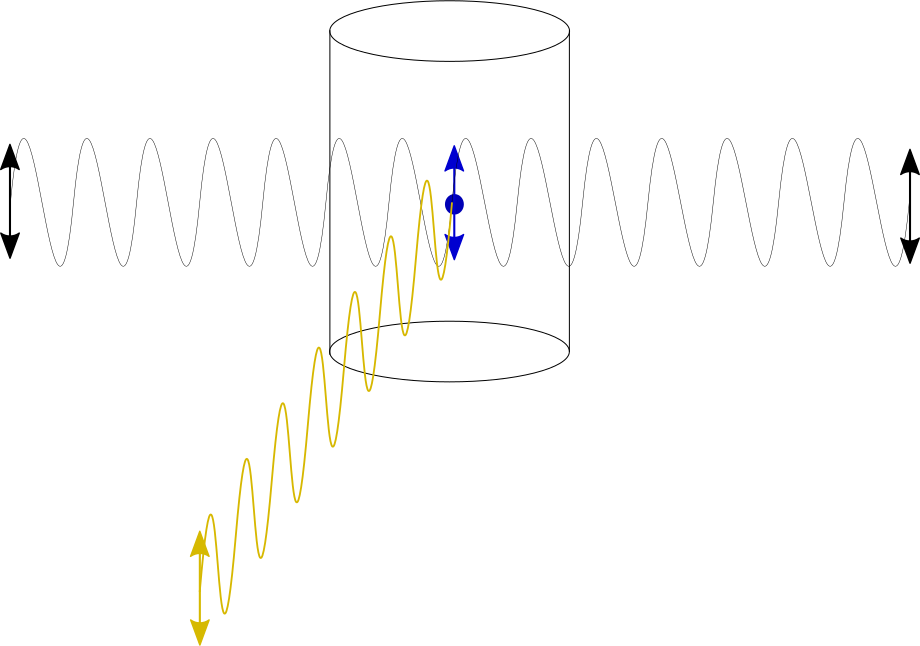
\includegraphics[height=.8\linewidth]{./img/pol_streu_vert.pdf}
		\caption[Vertikale Komponente]{Polarisation durch Streuung: Vertikale Komponente des unpolarisierten Lichtes}
	\end{subfigure}
	$\quad$
	\begin{subfigure}{.4\textwidth}
		\centering
		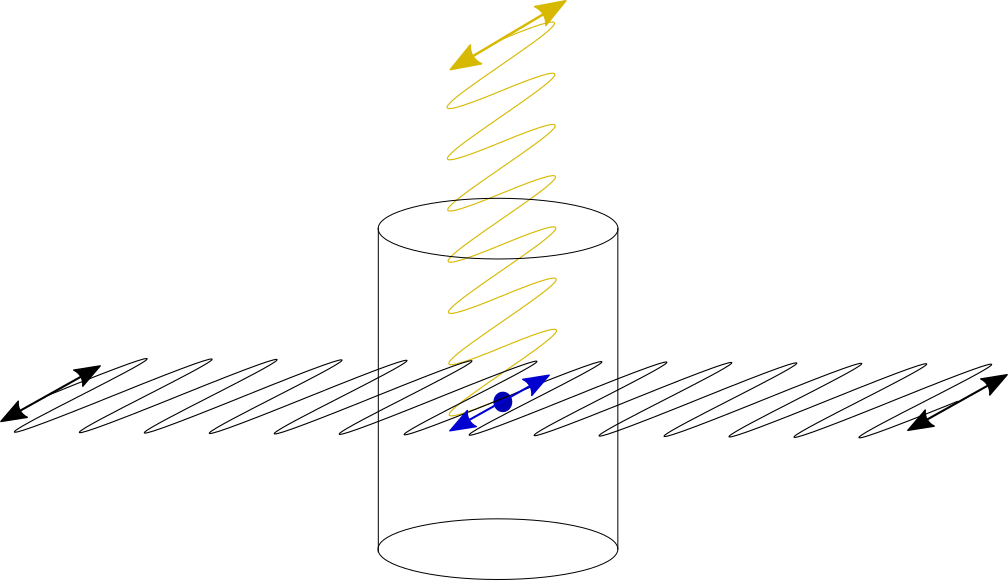
\includegraphics[height=.8\linewidth]{./img/pol_streu_hori.pdf}
		\caption[Horizontale Komponente]{Polarisation durch Streuung: Horizontale Komponente des unpolarisierten Lichtes}
	\end{subfigure}
	\caption[Visualisierung der Richtungsabhängigkeiten]{Abhängigkeit der Dipolstrahlung von der Richtung des einfallenden Lichtes}
	\label{fig:pol_streu}
\end{figure}

Zur Demonstration von Polarisation durch Streuung wird unpolarisiertes Licht auf ein Glas voll Wasser gerichtet.
Dabei wird das Licht mithilfe einer Blende möglichst gut zu einem Strahl geformt, welcher innerhalb des Wassers klar sichtbar ist.
Das durch das Wasser gestreute Licht wird mit einem Polarisationsfilter von verschiedenen Seiten beobachtet.
Dabei ist zu erkennen, dass das Streulicht aus verschiedenen Winkeln betrachtet unterschiedlich polarisiert ist.
Wird das Polarisationsfilter auf einer Stellung beibehalten, so kann aus einem bestimmten Winkel ein Intensitätsmaximum festgestellt werden, während bei einem zu diesem Winkel um \SI{90}{\degree} gedrehten Winkel nahezu kein Licht mehr sichtbar ist.
Daraus ist zu schließen, dass das einfallende unpolarisierte Licht durch die Streuung am Medium Wasser polarisiert wird.\par
Werden die Wassermoleküle als Oszillatoren aufgefasst, die von dem einfallenden Licht zu Schwingungen angeregt werden, so lässt sich das Phänomen erklären.
Durch die Anregung werden innerhalb der Moleküle Ladungen beschleunigt, welche ihrerseits eine Dipolstrahlung emittieren.
Diese wird vorzugsweise orthogonal zu ihrer Schwingungsrichtung ausgesendet, jedoch niemals entlang der Dipolachse.
Das so auslaufende Licht ist nahezu vollständig polarisiert, weshalb es nur mit einem Polarisationsfilter in der richtigen Stellung wahrgenommen werden kann.
